% !TEX root = ../KL-Projections.tex

%%%%%%%%%%%%%%%%%%%%%%%%%%%%%%%%%%%%%%%%%%%%%%%%%%%%%
\subsection{Optimal Transport Barycenters}
\label{sec-barycenters}

We are given a set $(\km{p})_{k=1}^K$ of input marginals $\km{p} \in \Si_N$, and we wish to compute a weighted barycenter according to the Wasserstein metric. This problem finds many applications, as highlighted in Section~\ref{sec-pw}.

Following~\cite{Carlier_wasserstein_barycenter}, the general idea is to define the barycenter as a solution of a variational problem mimicking the definition of barycenters in Euclidean spaces. Given a set of normalized weights $\la \in \Si_K$, 
we consider the regularized Wasserstein barycenter problem studied in~\cite{CuturiBarycenter}
\eql{\label{eq-barycenter-regul}
	\min_{p \in \Si_N} \enscond{ \sum_{k=1}^K \la_k W_\ga( \km{p},p ) }{ p \in \Si_N },
}
which as in~\cite{Carlier-NumericsBarycenters} can be re-written as 
\eq{
	\foralls k = 1,\ldots,K, \quad p = \pi_{k} \ones,
}
where the set of optimal couplings $\bpi = (\pi_{k})_{k=1}^K \in (\RR_+^{N \times N})^K$ solves
\eql{\label{eq-bary-variational-kl}
	\min \enscond{
		\KLdivL{\bpi}{\bxi} \eqdef \sum_{k=1}^K \la_k \KLdiv{ \km{\pi} }{\km{\xi}}
	}{
		\bpi \in \Cc_1 \cap \Cc_2	
	}
}
\eq{
	\qwhereq
	\forall k, \quad \km{\xi} \eqdef \xi \eqdef e^{ -\frac{C}{\ga} },
}	
and  the constraint sets are defined by
\begin{align*}
	\Cc_1 &\eqdef \enscond{ \bpi = (\km{\pi})_k \in (\Si_N)^K }{ \foralls k, \: \pi_{k}^T \ones = \km{p} } \\
	\qandq 
	\Cc_2 &\eqdef \enscond{ \bpi = (\km{\pi})_k \in (\Si_N)^K }{ \exists p \in \RR^N, \foralls k, \: \pi_k \ones = p }.
\end{align*}

It is easy to check that the Bregman iterative projection scheme can be applied to this setting by simply replacing $\KL$ by $\KL_\la$.

The $\KL_\la$ projection on $\Cc_1$ is computed as detailed in Proposition~\ref{prop-projkl-row-cols}, since it is equal to the $\KL$ projection of each $\km{\xi}=\xi$ on a constraint of fixed marginal $\km{p}$. 
The $\KL_\la$ projection on $\Cc_2$ is computed as detailed in the following proposition.

\begin{prop}\label{prop-klproj-bary}
	For $\bar\bpi \eqdef (\km{\bar\pi})_k \in (\RR_+^{N \times N})^K$, 
	the projection $\bpi \eqdef (\km{\pi})_{k=1}^K = \KLprojL_{\Cc_2}(\bar\bpi)$ satisfies
	\eql{\label{eq-projc2-bary}
		\foralls k, \quad
		\km{\pi} = \diag\pa{ \frac{p}{ \km{\bar\pi} \ones } } \km{\bar\pi}
		\qwhereq
		p \eqdef \prod_{r=1}^K ( \bar\pi_r \ones )^{\la_r}
	} 
	where $\prod$ and $(\cdot)^{\la_r}$ should be understood as entry-wise operators.
\end{prop}

\begin{proof}
	Introducing the variable $p$ such that for all $k$, $\pi_k \ones = p$, the first order conditions of the projection 
	$\KLprojL_{\Cc_2}(\bar\bpi)$ states the existence of Lagrange multipliers $(u_k)_k$ such that 
	\eq{
		\foralls k, \quad \la_k \log\pa{ \frac{\km{\pi}}{\km{\bar\pi}} } + u_k \transp{\ones} = 0 
		\qandq
		\sum_r u_r = 0. 
	}
	Denoting $a_k = e^{-u_k}$, one has $\prod_k a_k=\ones$ and $\km{\pi}=\diag(a_k^{1/\la_k}) \km{\bar\pi}$.
	Condition $\pi_k \ones = p$ thus implies that 
	\eq{
		a_k = \pa{ \frac{p}{\km{\bar\pi} \ones} }^{\la_k}, 
	}
	and condition $\prod_k a_k=\ones$ gives the desired value~\eqref{eq-projc2-bary}�for $p$.	
\end{proof}

\begin{rem}[Special case]
	Note that when $K=2$, $(\la_1,\la_2) = (0,1)$, one retrieves exactly the IPFP/Sinkhorn algorithm to solve the entropic OT, as detailed in Section~\ref{sec-entropic-regul}. Our novel scheme to compute barycenters should thus be understood as the natural generalization of this IPFP algorithm to barycenters.  
\end{rem}

\begin{rem}[Memory efficient and parallel implementation]
	Similarly as for Remark~\ref{rem-fast-sink}, one verifies that iterations~\eqref{eq-iter-bregmanproj}�in the special case of problem~\eqref{eq-bary-variational-kl} leads to iterates $\iter{\bpi} = ( \pi_k^{(n)} )_k$ which satisfy, for each $k$
	\eq{
		\pi_k^{(n)} = \diag(u_k^{(n)}) \xi \diag(v_k^{(n)})
	}
	for two vectors $(u_k^{(n)},v_k^{(n)}) \in \RR^{N} \times \RR^N$ initialized as $v_k^{(0)} = \ones$ for all $k$, 
	and computed with the iterations
	\eq{
		u_k^{(n)} = \frac{p^{(n)}}{\xi v_k^{(n)}}
		\qandq
		v_k^{(n+1)} = \frac{\km{p}}{ \transp{\xi} u_k^{(n)}}
	}
	where $p^{(n)}$ is the current estimate of the barycenter, computed as
	\eq{
		p^{(n)} = \prod_{k=1}^N \pa{ u_k^{(n)} \odot (\xi v_k^{(n)}) }^{\la_k}.
	}
	A nice feature of these iterations is that they can be computed in parallel for all $k$ using multiplications between the matrix $\xi$ and matrices storing $(u_k^{(n)})_k$ and $(v_k^{(n)})_k$ as columns. 
\end{rem} 



Figure~\ref{fig-barycenter-entropic} shows an example of barycenters computation for $K=3$.	The three vertices of the triangle show the input densities $(p_1,p_2,p_3)$ which are uniform on binary shapes (diamond, annulus and square). 
The other points in the triangle display the results for the following values of $\la$
\eq{
	\begin{tabular}{c}
		(0,0,1) \\
		(1, 0, 3)/4 \quad (0, 1, 3)/4 \\
		(1,0,1)/2 \quad (1,1,2)/4 \quad (0,1,1)/2 \\ 
		(3,0,1)/4 \quad (2,1,1)/4 \quad (1,2,1)/4 \quad (0,3,1)/4 \\
		(1,0,0)\quad (3,1,0)/4 \quad (1,1,0)/2 \quad (1,3,0)/4 \quad (0,1,0)
	\end{tabular}
} 
The computation is performed on an uniform 2-D grid of $N = 256 \times 256$ points in $[0,1]^2$, and $\ga=2/N$.

\begin{figure}[h!]
	\centering
	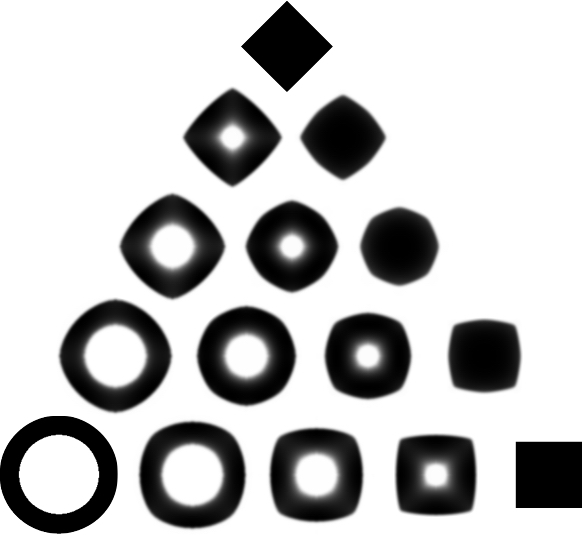
\includegraphics[width=.7\linewidth]{barycenters/shapes}
	\caption{% 
		Example of OT barycenters with entropic smoothing. 
		%		
	}
   \label{fig-barycenter-entropic}
\end{figure}

We benchmark the performance of the Bregman iterative projection scheme to compute barycenters with the approaches proposed in~\cite{CuturiBarycenter} and~\cite{Carlier-NumericsBarycenters}. We propose for this benchmark to compute the quadratic-Wasserstein barycenter of $K=12$ probability histograms on the $N=100\times 100$ planar grid. These histograms are obtained as discretized and then renormalized truncated mixtures of Gaussians on the grid, as displayed in Figure~\ref{fig-barycenter-inputmeasures}. We consider for the $N\times N$ cost matrix $C$ the matrix of squared Euclidean distances on the grid, normalized to have median $1$.

\begin{figure}[h!]
	\centering
	\includegraphics[width=\linewidth]{barycenters/input_measures}
	\caption{% 
		Input measures considered in our experiment. They are formed by considering truncated mixtures of Gaussian densities on the planar square, which are then discretized on a regularly spaced $100\times 100$ grid and normalized as histograms in $\Sigma_{10^4}$.
		%		
	}
   \label{fig-barycenter-inputmeasures}
\end{figure}


We review briefly two competing methods for this task. The authors of~\cite[\S5]{CuturiBarycenter} proposed to minimize directly Equation~\eqref{eq-barycenter-regul} with a regularizer $\varepsilon>0$. That objective can be evaluated by running $K$ Sinkhorn fixed-point iterations. That objective is differentiable and its gradient is equal to $\varepsilon\sum_k \la_k \log u_k$, where the $u_k$ are the left optimal scalings obtained with the Sinkhorn subroutine, run in parallel. The cost of each iteration of the Sinkhorn algorithm is $2KN^2$, namely the cost associated to the updates of row and column scalings, each obtained by multiplying a $N\times N$ matrix (the kernel $\xi$) times a $N\times K$ matrix (a matrix of scalings). A weakness of that approach is that a precision threshold $\tau$ for each Sinkhorn fixed-point sub-iteration must be chosen. That precision can be measured by the difference in $l_1$ norm between the row and column marginals of $\diag(u_k)\xi\diag(v_k)$ and the target marginals. Setting that tolerance $\tau$ to a larger value ensures a faster convergence of the subroutine but results in noisier gradients. We experiment here with two thresholds $\tau\in\{0.01,0.1\}$ and set a constant gradient stepsize $t_0$ to $1$. The authors of~\cite{Carlier-NumericsBarycenters} propose to solve directly the (non-differentiable) energy of Equation~\eqref{eq-barycenter-regul} when $\varepsilon=0$. They study a dual formulation for that energy that involves splitting across dual variables and show that subgradients of the energy for each of these $K$ dual variables can be computed in closed form by solving $K\times N$ nearest neighbor assignments (among $N$ neighbors) on a shifted metric. They propose to use a L-BFGS method that exploits directly such subgradients, which we implement in practice using Matlab's \texttt{fmincon} function. At each step of their algorithm, iterates in the primal can be obtained by averaging all of the $K$ subgradients.


\begin{figure}
	\centering
	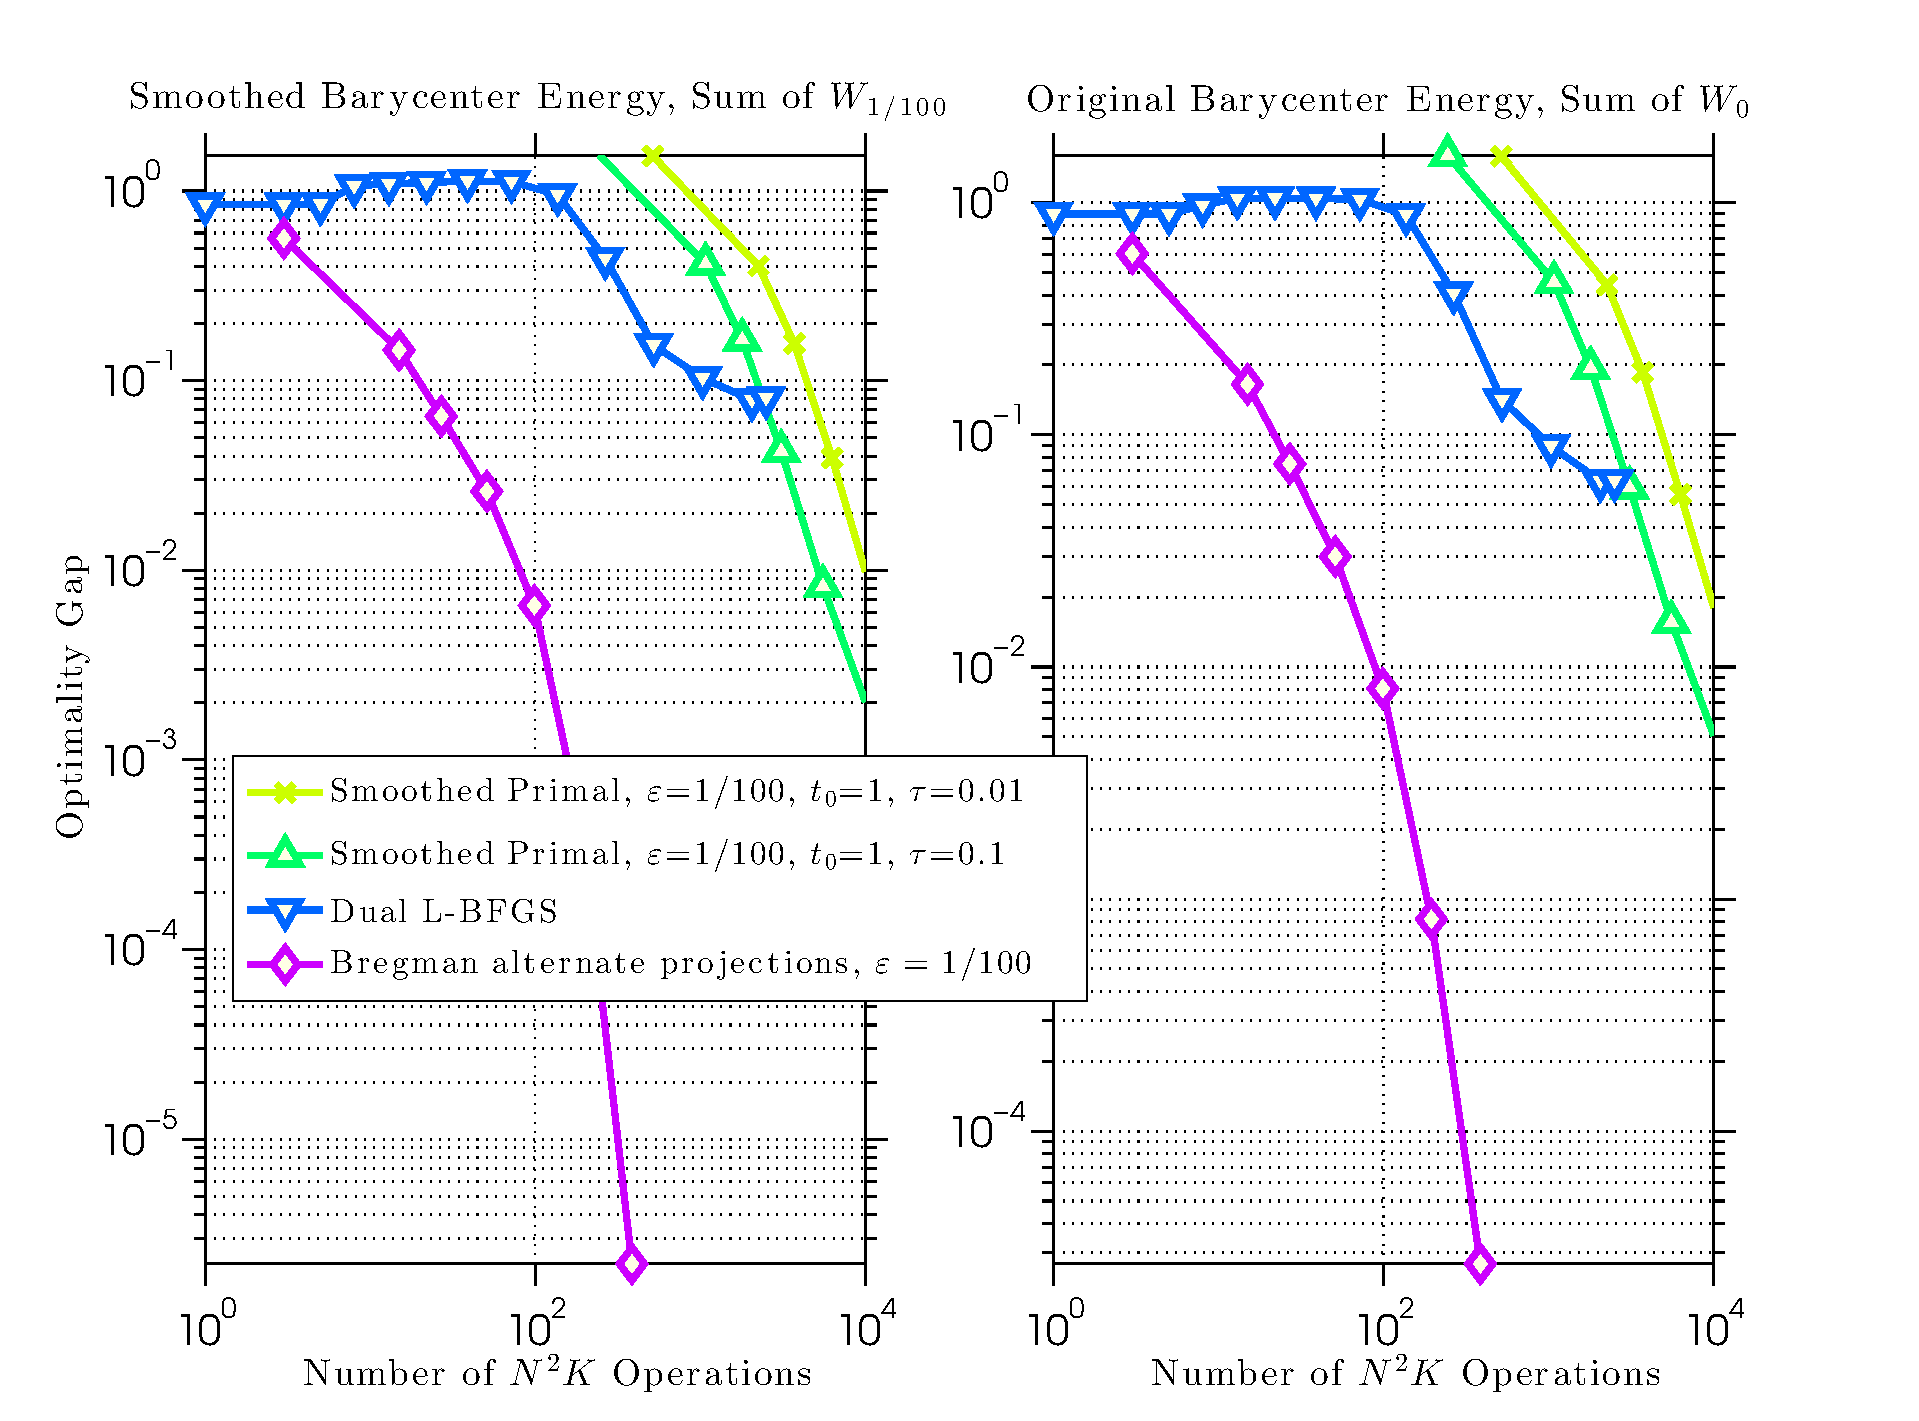
\includegraphics[width=\linewidth]{barycenters/bregvsrest4}
	\caption{Optimality gap as a function of the number of iterations (each consisting in $N^2K$ operations) of the three considered methods with respect to both the smoothed Wasserstein energy that involves a sum of $K$ smoothed distances $W_{1/100}$ terms, and the original Wasserstein barycenter energy involving sums of $W_0$ terms. The smoothed primal descent approach of~\cite{CuturiBarycenter} is considered here with two different tolerance parameters $\tau$ that control the convergence of the Sinkhorn subroutine used in that algorithm. We set the smoothing parameter $\varepsilon$ to $1/100$, having renormalized the matrix of squared Euclidean distances between all nodes on the grid to have a median of $1$. Notice that both $x$ and $y$ axis are displayed in logarithmic units. The Bregman alternative projection approach advocated in this paper converges orders of magnitude faster.}
   \label{fig-barycenter-gaps}
\end{figure}

Because our approach as well as that of~\cite{CuturiBarycenter} on the one hand, and that of~\cite{Carlier-NumericsBarycenters} on the other hand, minimize two different energies---the sum of $K$ smoothed distances $W_\varepsilon$ and the sum of $K$ original Wasserstein distances $W_0$ respectively---comparing them on only one of these two energies does not make sense. We plot in Figure~\ref{fig-barycenter-gaps} the gap to optimality of each method with respect to smooth ($\varepsilon=1/100$) and non smooth energies as a function of the number of iterations consumed by the algorithm. By gap to optimality we mean in the $y$ axis the difference between the objective evaluated at the primal iterate and the optimal value for that problem, after $x$ iterations in the $x$ axis.  We consider as a proxy for the optimal value the smallest value obtained across all methods after $10^5$ iterations. This minimum across all methods is in fact attained much earlier by the Bregman alternated projections approach after only 771 iterations (we do not plot that point in our graph), which is set to terminate when the $l_1$ norm of two successive iterates is less than $10^{-8}$. By one iteration, we mean an iteration whose cost is equal to $N^2K$ elementary operations. The number $N^2K$ corresponds to the $K$ matrix-vector products of cost $N^2$ needed by both the Sinkhorn subroutine or the Bregman alternative projections, or $K\times N$ nearest-neighbor assignments involving $N$ candidates carried out in the dual descent. A perhaps surprising observations from these experiments is that the minimizer of the smoothed energy ends up providing, using either smoothed primal descent or Bregman iterations, a better minimizer of the non-smoothed energy as well. This is certainly due to the fact that we apply a relatively small smoothing $\varepsilon=1/100$, and partly due to the tolerance and convergence criteria we have applied to the dual L-BFGS method. This reflects however the fundamental inability of the dual L-BFGS method to solve with a subgradient descent what is essentially a very large and degenerate linear program. 

The barycenters we obtain for each of the three methods are displayed in Figure~\ref{fig-barycenter-bars}. We only report the barycenters as they appear after at most $10^4$ iterations. The barycenter obtained after more than $10^5$ iterations with the smoothed primal descent approach of~\citep{CuturiBarycenter} (not plotted here) is identical to that obtained with the Bregman iterative projection scheme, which should be expected since they minimize the same energy.

\begin{figure}[h!]
	\centering
	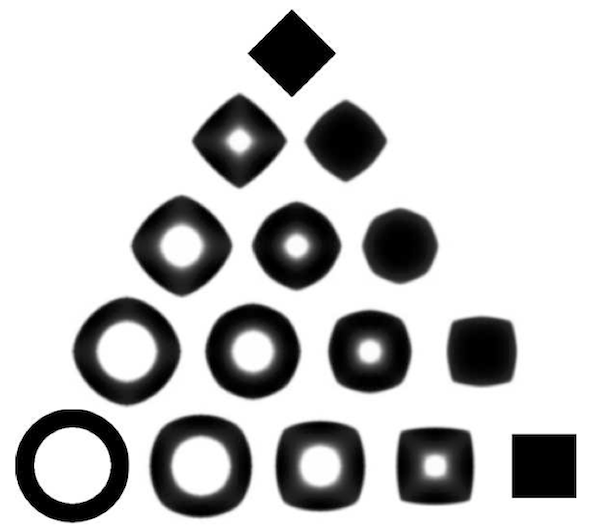
\includegraphics[width=\linewidth]{barycenters/barycenters}
	\caption{% 
		Isobarycenters obtained with three different methods for the input measures displayed in Figure~\ref{fig-barycenter-inputmeasures} after up to $10^4$ iterations. The Bregman barycenter is obtained with a couple of hundred iterations.
		%		
	}
   \label{fig-barycenter-bars}
\end{figure}


